\Lecture{Jayalal Sarma }{ 2 october, 2020}{11}{More on PIE, PIE -Tuttes-Matrix-Tree-Theorem-Part2}{Shrinidhi Bajpayee}{$\alpha$}{JS}



\section{Introduction}
We finished Tutte's Matrix Tree Theorem in non trivial way.Let's just recall Tutte's Theorem.We have directed graph $G(V,E)$.We have $V={v_1,v_2,....v_n}$.\\
A $n \times n$ matrix $L(G)$ called the \textit{Laplacian matrix} of $G$ as follows.
\[
  L(G)_{ij} =
  \begin{cases}
    indeg(v_i) & \mbox{ if } i = j,                                     \\
    $$ $$ -1   & \mbox{ if }~ i \neq j ~\text{and}~(v_i,v_j)\in E$$  $$
    $$ $$ 0    & \mbox{ otherwise (When there is no edge) } $$ $$
  \end{cases}
\]
What theorem says,the number of spanning arborescences rooted at some vertex n is given by exactly equal to $det(L_G[i])$ Here i=n.\\
Quickly Recap Definition of Spanning arborescences :An \textit{Arborescence} is a directed graph in which a vertex $u$ is called the root and for every other vertex $v$ in the graph, there is exactly one directed path from $u$ to $v$. In simpler terms, an arborescence is an directed tree in which all the edges are directed away from the root. A \textit{Spanning Arborescence} $S(V,E)$ of a directed graph $G(V',E')$ is an arborescence such that $V=V'$ and $E\subseteq E'$.\\
One condition is that there is a directed path from V to every vertex in G within E'.\\
Second condition is underlying undirected graph should be a tree. \\ \\
Let's just take away of Last Lecture .\\
One take away is as following:\\
\begin{align}
  det(L_G[n]) = \sum_{\sigma \in S_{n-1}}~
  Sign(\sigma)~\prod_{i=1}^{n-1}L_{i\sigma(i)}
  \label{eq:to_prove:Tutte}
\end{align} \\
$S(n-1)$ is notation for permutation of $n-1$.\\
This is expression of determinant that we have seen in last lecture.\\
So we want to show it is equal to spanning arborescence we introduce concept called Spreg.So what is Spreg $?$.\\
We quickly define Spreg.\\
\begin{definition}\textbf{Spregs:} Single prdecessor graphs or \textit{Spregs} with distinguished vertex $v$ of a directed graph $G(V,E)$ is a subgraph $T(V,E')$, $E' \subseteq E$, such that each vertex in $T$ except the vertex $v$ has exactly one predecessor and the vertex $v$ has no predecessors. In other words; in the spreg T, $indeg(v) = 0$ and for every $u \neq v$, $indeg(u)=1$.\\
\end{definition}\\
Every vertex other than distinguished vertex must be indegree 1.Subgraph of G is called Spregs.So there are several spregs are possible similar to several spanning arborescence possible.\\
We want to count spanning arborescence using spregs.That will be very nice combinatorial interpretation of this topic,that is plan.\\

1. We want to count the number of spanning arborescence rooted at Vn.\\ \\
2.We want to count the number of spregs distinguished vertex Vn.\\
We associated with last lecture that every spanning arborescence corresponds to spregs .It turns out there are more spregs.There is some structure,Spregs looks like are of the form arborescence $+$ weekly connected component 1 $+$ weekly connected component 2......\\
V can not be part of cycle.V can be vertex in component.Weekly connecetd component has exactly 1 cycle.\\
So what we want to count spregs in inner circle with distinguished vertex Vn.Ok so already know what we have to count.Basic strategy is as follows:\\
Strategy is that count the number of spregs with distinguished vertex Vn which does not have any cycle.So this is what we want to count.We want to use Inclusion Exclusion.In fact we will not only count through Inclusion exclusion but we will go through each term of the determinant expression corresponds to our counting terms.\\
Let's demonstrate by writing down Inclusion exclusion.\\
In order to define Inclusion Exclusion formulation we need to define the \\ \\
1.Universe (Called as X).\\
2.Component $A_i$.\\
To define that Let's consider,notice that we want to count spregs without any cycle.\\
We need to be set of all spregs with distinguished vertex $V_n$.\\
Let $C_1,C_2,C_3, \dots , C_n$ be the set of cycles in graph G.We looking at simple cycle.\\
$A_i$ define as spregs which contain the cycle $C_1$.The number of spregs which does not contain any cycle.This what we want to count.So,\\

$|X|$ $-$ $|\bigcup_{i=1}^{n} A_i|$\\
It is same as,
&=$$|X| - \sum_{I \subseteq [n] , I \neq \emptyset} (-1)^{|I|+1}|\bigcap_{i \in I} A_i|$$\\
So already applied Inclusion Exclusion,Now write it as
&=$$ |X| + \sum_{I \subseteq [n] , I \neq \emptyset} (-1)^{|I|+1}|\bigcap_{i \in I} A_i| $$\\
So basically we need to count this.We can say that each term in these expression are exactly same as term used in determinant expression.As number of Spregs are equal to number of spanning arborescence,hence theorem is called.This is strategy.Hence each term is associated with terms of determinant theorem.\\
\textbf{Observation:}Let's consider C1,C2 be two cycles.\\
What can say about $$ A1 \bigcap A2 = \emptyset iff C1
  \bigcap C2 \neq \emptyset.$$\\
Every spregs looks like arborescence + uniquely weekly connected component 1 +uniquely weekly connected component 2.\\
$$ If C1 \bigcap C2 \neq \emptyset then |A1 \bigcap A2| =0.$$\\
Using the observation,\\
The number of spregs with distinguished vertex Vn which is acyclic is nothing but \\
&= $$ |X| + \sum_{I \subseteq [n] ,I \neq \emptyset ,for J,K \belongs I, J \neq K, cj \bigcap ck =\emptyset}       (-1)^{|I|+1}|\bigcap_{i \in I} A_i| $$\\

\textbf{Recall:} We counted |X| =Total number of spregs\\
$$det(L_G[n]) = \sum_{\sigma \in S_n} Sign(\sigma)  \prod_{i=1}^{n} a_{i\sigma(i)}$$\\
This is determinant expression.\\
&= term   corresponds   to   $$ \sigma=id $$\\
&= $$\prod_{i=1}^{n-1} (L_i) = \prod_{i=1}^{n-1} deg_in(L_i) $$\\
Now we count the singleton sized I.\\
Spregs that contain exactly one cycle.\\
Fix,I={1},We are counting spregs which contain only C1.\\
Let  CI be (Vi1,Vi2,Vi3,....Vin)\\
$$\sigma(i1)=i2$$\\
$$\sigma(i2)=i3$$\\
$$\sigma(ik-1)=ik$$\\
$$\sigma(ik)=iI$$\\
$$\sigma \in S_n-1$$\\
$$\forall other  i \in {1...n} $$\\
$$ \sigma(i)=i $$\\
This is permutation which contain one cycle.\\
Now we just able to do following\\
\textbf{Claim:} Term in the determinant expression for\\
$$LG[n] corresponds to \sigma=number of spregs which contain C1$$ \\
Right now we are talking about one circle.\\
Let's see proof of this.\\
Proof of this is very natural.
$$sign(\sigma)\prod_{i=1}^{n-1} L_i,\sigma(i   $$\\
sign of permutation is exactly equal to
$(-1)^{(l-1)} $.Here length is l.\\
Second term is \\
$$ (-1)^{(l-1)} (\prod_i,|\sigma(i)|=i L_i,i)(\prod_i,|\sigma(i)| \neq i L_i,\sigma(i)) $$\\
$$ L_i,\sigma(i) =-1,if V_i,V_\sigma(i) is edge in graph \in E\\ ootherwise  $$\\
If corresponding edge is present then this term is non zero otherwise zero.\\
$$ (-1)^{(l-1)}(\prod_i,|\sigma(i)| deg_in(v_i))*(-1)^{l} $$\\
$$&= (-1)^{(2l-1)} |number of spregs which contain C1|  $$\\
$$&= -|number of spregs which contain C1 | $$\\
Proposition for $$ \sigma \in S_n-1 comsisting of single cycle.   $$\\
$$ \sigma =(i1,i2,.....il)   $$\\
Associate$ C\sigma $ as a cycle corresponds to vertex sequence (Vi1,Vi2,Vi3.....Vil,Vii)\\
Then the term in the determinant corresponds to $\sigma$ satisfies following.\\
$$sgn(\sigma)(\prod_{i=1}^{n-1}L_i,\sigma(i))$$

$$ &= -(\prod_{i,\sigma(i)=i}deg_in(v_i))C_\sigma \subseteq G(V,E) $$\\
$$ 0 if C\sigma \nsubseteq G(V,E) $$ \\
$$-1  if C\sigma \subseteq G(V,E) if \forall i \sigma(i) \neq i     $$\\


\textbf{Corollary:}$$For \sigma,C\sigma as above $$\\
$$ |\prod_{i=1}^{n-1}L_i,\sigma(i)|=number of spregs which contain C_\sigma   $$\\
Now this is case for single cycle.\\Now we will generalise case for multiple cycle.\\
So it is very natural.\\
\textbf{Question:}Suppose $\sigma$ \in $S_n-1$ is the product of K>0 disjoint cycle.\\
$$\sigma=(i11,i12,i13.....iil) (i21,i22,i23....(ikl,ik2,ik3...ikl)    $$
K is number of cycles.\\
So now we are associate \\
$$ C_\sigma = \cup  {j=1}^{k}C_j  where C_j is ()V_ij1....V_ijLj.....VijI)$$\\
Then the term  corresponds to $\sigma$ in $det(L_G[n])$\\
$$sgn(\sigma) = (-1)^{K} \prod_{i|\sigma(i)|}deg_in(V_i) if C_\sigma \subseteq G   $$\\
$$ o if C\sigma \nsubseteq G $$

\textbf{Corollary:}If we look at\\
$$|\prod_{i=1}^{n}L_i,\sigma(i)|=number of spregs which contain C_\sigma = \bigcup_{j=1}^{k}C_j   $$\\
$$ det(L_G[n]) =\sum_{\sigma \in S_n-1}sig(\sigma) \prod_{i=1}^{n} L_i\sigma      $$\\
This is how determinant expression looks like.\\
Number of spanning arborescence rooted at Vn  as distinguished vertex and not containing cycle.\\
$$&=|X| + \sum_{I \subseteq [n] ,I \neq \emptyset, cj \bigcap ck=\emptyset ,j,k \in I}(-1)^I    $$\\
This is strategy.
This lecture is combinatorial application of PIE.

\newpage
WEEK 4 LECTURE 2\\
Algorithmic Application of PIE
\section{Introduction} We talk about counting problem.Its about given a $n*n$ bipartite graph,We want to count the number of perfect matching in it?\\
subset of edges such that every vertex has exactly one edge incident on it from the
subset.\\
Bipartite adjacency matrix is different from adjacency matrix.\\ \\
\textbf{Trivial Algorithm:}Run through all n sized subsets of E.\\
$${n^{2} \choose n } \sim {n^{2} \choose n}^{n}    \sim n^{n} \sim 2^{nlogn}$$\\

$$ {n \choose k}^{k} \leq {n \choose k} \leq {n_e \choose k}^{k} $$\\
e=natural log base \\
\section{Decision Problem:}
\textbf{Binpacking Problem:}
Given a positive integer (bin capacity B),positive integer k\\
We have n item with weight S1,S2,S3.....,Sn\\
partition the items into u1,u2,u3.....,uk\\
Capacity is such that sum of weights of items in each ui is almost B.\\
This is binpacking problem.\\
It is NP-problem.\\
By PIE Time complexity is $O(nB2^{n})$\\
n=number of items\\
B=capacity\\
Now we will reformulate PIE.\\

Given a collection of N combinatorial objects \\
Let p(1),p(2),p(3)...p(n) be properties.\\
$p_i$ is essential function \\
$$ N \to {0,1}   $$\\
It is possible that some object doesn't have properties of that.\\
$$N_i \to Number of objects among N with property P(i).$$\\
$$ {i_1,i_2,....i_r} \subseteq {1,2,3,...N} $$\\
$$N_i_1,i_2,i_3....i_r = Number of objects with properties p(i_1) p(i_2)....p(i_r) $$\\
N(0)=Number of objects not having any of the property.\\
$$ N(0)=N-\sum_{i=1}^{n} N_i_1 +\sum_{i_1<i_2}N_i_1,i_2 -\sum_{i_1 < i_2 <i_3}.......(-1)^{j} \sum_{i_1<i_2<...i_j}N_i_1,i_2...i_j (-1)^{x}N_1...r   $$\\
Restatement (Complementary term)(For the discussion)\\
$$N \to Number of objects.$$\\
$$Q(1),Q(2),....Q(n) $$be properties that some of these objects have.\\
$$W \subseteq {1,2,....n}  $$\\
Let N(W) be the number of objects having none of the properties Q(i).\\
$$i \in W   $$\\
Now what we want to count the other set.\\
$$X \to number of objects which has all the properties.$$\\
$$X = \sum_{W \subseteq [n]}(-1)^{|W|} N(W)   $$\\
\textbf{Pf:}$Define P(i) iff \neg Q(i)$\\
Now the above restatement is applicable.\\
Given a bipartite graph $G(u,v,E)\\
  |u|=|v|=n $\\
count the number of perfect matching.\\
\textbf{I/p:}Bipartite adjacency matrix.\\
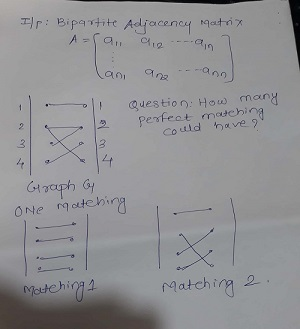
\includegraphics{graph.jpg}\\ \\
There are 2 perfect matching is in these graph.\\
Matching 1: There is bijection.\\
There are 4!=24 permutation.But matching 1 and matching 2 are two permutation for perfect matching.\\
How's the algebric way of writing itself.\\
Let's write $\sigma \in S_n$ \\
Consider,\\
$$ \prod_{i=1}{n} a_i \sigma(i)$$\\
When $a_i \sigma_i$ is non zero value.
When $i\sigma _i$ is true.\\
$$\prod a_ii = a11 .a22 .a33. a44$$\\
$$ &=1 $$\\
What will be product of \\
$$\prod_{i=1}{n} a_i \sigma(i) $$\\
$$ &=a12. a21.a33.a44  $$\\
$$ &=0  $$\\
If corresponding edge is there in graph then value will be 1 otherwise 0.\\
a12=0 since no edge from 1 to 2.\\
Let's write,\\
Permanant of A=\\
$$ \sum_{\sigma \in S_n}  = Number of perfect matching in the graph.$$\\
Given a matrix A,\\
Its two types are:\\
!)permutataion (A) that is per(A): It is number of perfect matching in graph.\\
2)Determinant (A) that is det(A)\\
\\
\textbf{Problem:}Given a matrix A o/p the value of per(A)\\
\textbf{Trivial Algorithm:}Run over all $\sigma \in S_n$ compute the product \\
$$\prod_{i=1}{n}a_i \sigma(i)$$ and add.\\
$$O(n!) \sim O(n ^{n}) \sim 2^{nlogn} $$\\
\textbf{Lemma:}A is bipartite adjacency matrix of a bipartite graph G\\
$$Per(A) = \sum_{W \in {1...n}}(-1)^{|W|} \prod_{i=1}^{n}(\sum_{j \notin W}a_ij)$$\\
Applying Lemma,\\
$2^{n}$ W's and n^{2}=remaining Computation\\
2^{n}n^{2} time algorithm.\\
\textbf{PF:}To apply complementary form PIE.\\
Define N objects: M \in N\\
M \subseteq E such that for  every \\
$\forall i \in {1...n}$ the vertex $X_i$ is the endpoint of some vertex in M.\\
$\forall j \in [n] Q(j)$: Vertex $Y_j$ is the endpoint of some vertex in M.\\
We want to count number of objects from underlined part which satisfies Q(1) .....Q(n)\\
The number of perfect matching=per(A)=number of objects which satisfies all of Q(1) Q(2)....Q(n)\\
Q(1) says first one is matched.\\
Q(2) says second one is matched.\\
Like this etc etc.\\
When all vertex are matched from both side.\\
$$ &= \sum_{W \in {1...n}}(-1)^{|W|}$$\\
N(W)=Number of objects which satisfies none of property in W.\\
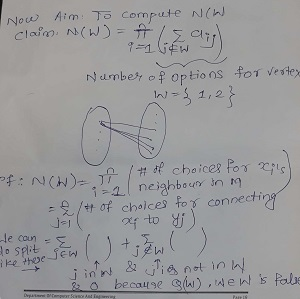
\includegraphics{img.jpg}\\ \\
Per(A)=Number of perfect matching.\\
$$ &=\sum_{W \subseteq {1...n}}(-1)^{|W|}(\prod_{i=1}^{n}(\sum_{j \in w}aij)) $$\\
This completes the proof of the Lemma.\\
This lemma gives O(2^{n}n^{2}) algorithm for computing number of perfect matching in a given bipartite graph.\\
NP complete=Decision Problem.\\
#p(partly)complete=counting complexity.\\
\textbf{Quickly Recap:}\\
\textbf{Binpacking problem:}\\
$Bin capacity B,We have number of bins K,We have n items S1....Sn are sizes.$\\
$Question is Can we partition items to u1....uk[n]such that$\\\
$$\forall_{$i\leq j \leq k}j\sum_{i \in u}Si \leq B$   $$\\
  We want to count this.\\
  \textbf{Algorithm:}\\
  \textbf{Trivial Algorithm:}Run through partition.\\
$$ n \choose k$$\\
O(nB2^{n}) time space.\\
A partition of [n] into u1....uk is said to be feasible if the sum of the sizes of item $\leq$ B in uj.\\
\textbf{Relax:}Items can appear more than once.\\
\textbf{observation:}A feasible solution with relaxation will remain feasible without relaxation.\\
\textbf{Relaxed Solution:}ordered set of K lists of items from {1...n}.\\
1.Each of the elements in {1...n}appears atleast in one list.\\
2.For each list a1,a2....ap
$$\sum_{h=1}{p}S_ak \leq B $$\\
To apply PIE,we need to define objects Q1....\\
\textbf{Objects:}Ordered sets of K list of elements from {1...n} such that for each list (a1...ap) $$\sum_{h=1}{p}S_an \leq B $$\\
Q(1):=The ordered list of k lists contain 1 in atleast one list in it.\\
.\\
.\\
.\\
Q(W):=W  is contained in atleast one of the lists in the ordered set of list.\\
.\\
.\\
.\\
Q(n)\\
X=Set of objects which satisfy all of the properties Q(1)....Q(n)\\
$$X=\sum_{w \subseteq [n]}(-1)^{|w|} N(W) $$\\
\textbf{Aim:}To compute N(W)\\
A(W):=Number of list a1....ap of elements list in W.\\
$$ \sum_{h=1}{p}S(an) \leq B $$\\
$$N(W)=(A(W))^{k}  $$\\
\textbf{Aim:}Compute A(W)\\
$P_w(j)$ =number of list a1....ap of which element not in w such that
$$\sum_{h=1}{p}S(ak)=j  $$\\
$$A(w)=\sum_{j=0}{B}P_w(j)$$\\
$$P_w(j)=\sum_{i \notin w}P_W(j-s(w)) $$\\
$$ p_W(j)=0, j<0 $$\\
$$P_w(0)=1 $$\\
Time taken is O(nB2^{n})


% Lecture 3


\Lecture{Jayalal Sarma}{Oct 10, 2020}{13}{From Principle of Inclusion-Exclusions to Mobius Inversion}{Sandip Saha}{$\alpha$}{JS}

% \section{Introduction}
The journey so far has been that we have started with pigeon hole principle and its applications then we used double counting and bijections to establish different identities then we moved to PIE and its different applications.
% Then we came to Principle of Inclusion-Exclusion(PIE) as a consequence of a bijection argument. 
In this lecture, we will look at a more generalized version of PIE and move gradually towards the Mobius Inversion.

\subsection{PIE Revisited}
Previously we have used PIE to compute $\left| \bigcup^n _{i=n} A_i \right|$ as follows,
\[ \left| \bigcup^n _{i=n} A_i \right|=\sum_{\emptyset \neq I \subseteq [n]} (-1)^{|I|+1}\left|\bigcap_{i\in I} A_i\right|\]
Now, we are interested to compute $\left|\bigcap_{i=1}^n  \overline{A_i}\right|$, which can be rewritten as,
\begin{align}
  \left|\bigcap_{i=1}^n  \overline{A_i}\right| & = \left|
  \overline{\bigcup_{i=1}^n  A_i}
  \right| \nonumber \tag{using De-morgan's law}                                                                                                                    \\
                                               & = \left| X \right| - \left| \bigcup^n _{i=n} A_i \right| \nonumber                                                \\
                                               & = \left| X \right| -\sum_{\emptyset \neq I \subseteq [n]} (-1)^{|I|+1}\left|\bigcap_{i\in I} A_i\right| \nonumber \\
                                               & = \sum_{ I \subseteq [n]} (-1)^{|I|}\left|\bigcap_{i\in I} A_i\right|
\end{align}

Note that $\bigcap_{i\in \emptyset} A_i =X$. This thing can also be stated in the following way.

\begin{theorem}
  Let $X$ be a finite set and $P_1,\dots, P_m$ properties. Further define for $S \subseteq [m]$ the set $N(S) = \{x\in X \mid \forall i \in S: x \text{ has property } P_i\}$  then, number of elements in $X$ satisfying none of the properties $P_1,\dots, P_m$ is given by,
  $$ \sum_{S \subseteq [m]} (-1)^{|S|} \left| N(S) \right|$$
\end{theorem}

\subsection{Stronger version of PIE}
The Inclusion-Exclusion Principle has a stronger version which is as follows.

\begin{theorem}[Stronger PIE]
  \label{stronger PIE}
  Let $f,g:2^{[n]}\longrightarrow \mathbb{R}$ are functions assigning real numbers to subsets of $[n]$ with the property that for any $A\subseteq [n]$

  \[ g(A)=\sum_{S\subseteq A} f(S)\]

  Then,
  \[ f(A) = \sum_{S \subseteq A} (-1)^{|A|-|S|}g(S)\]

\end{theorem}


\begin{proof}
  Let $f$ and $g$ are functions from the powerset of $[n]$ to real numbers and for all $A \subseteq [n]$
  \[g(A)=\sum_{S\subseteq A}f(S)\]

  \begin{align}
    \sum _{s\subseteq A}( -1)^{|A|-|S|} g( S) & =\sum _{s\subseteq A}( -1)^{|A|-|S|}\left(\sum _{T\subseteq A} f( T)\right) \nonumber \\
                                              & =\sum _{T\subseteq A} C_{T} f( T)
  \end{align}
  Where $C_T$ is appropriate signed number. Our aim is now to find $C_T$ for different $T$

  \begin{description}
    \item{\textbf{Case 1: }($T=A$)} $C_T=1$, since $f(A)$ is only encountered for $T=S=A$.

    \item{\textbf{Case 2: }($T \neq A$)} choosing a set between $T$ and $A$ is equivalent of choosing a set from $A\setminus T$
          \[C_T=\sum _{T \subseteq S\subseteq A}( -1)^{|A|-|S|}=\sum^k_{i=0}(-1)^{k-1} {k \choose i} =0 \]
  \end{description}
  This proves the claim.
  \[\boxed{\therefore f(A) =  \sum_{S \subseteq A} (-1)^{|A|-|S|}g(S)}\]
\end{proof}

\textbf{Why it is strong version?} it implies PIE.
Assume the strong version, we can derive PIE.
\begin{proof}
  Properties $P_1,\dots, P_m$ of elements of $X$ . $X_1,\dots, X_m$ are the subsets of $X$ satisfying the respective property i.e. $X_i=\{ x\in X \mid x \text{ satisfy } P_i\}$.
  then for $S \subseteq [m]$  we define $f(S)$ to be the number of elements in $X$ having all properties $P_i$ such that $i \notin S$ and none of the properties $P_j$ such that $ j \in S$ i.e.
  \[ f(S) = \left| \bigcap_{i\in [m] \setminus S} X_i \setminus \bigcup_{i\in S} X_i \right| \]
  We are interested in counting the number of elements in $X$ which does not satisfy any property in $P_1,\dots, P_m$ i.e. $f([m])$. We define,

  \begin{align*}
    g(A) & = \sum_{S\subseteq A} f(S)                         \\
         & = \left| \bigcap_{i \in [m] \setminus A}X_i\right| \\
         & = N([m]\setminus A)
  \end{align*}
  $g(A)$ counts $x\in X$ if the property that $x$ does not satisfy forms a subset of $A$. By \ref{stronger PIE}
  \begin{align*}
    f([m]) & = \sum_{S\subseteq [m]}(-1)^{m-|S|} g(S) \\
           & = \sum_{\substack{
    S'\subseteq [m]\setminus S                        \\
        S\subseteq [m]}}
    (-1)^{|S'|} N(S')                                 \\
           & = \sum_{S \subseteq [m]} (-1)^{|S|} N(S)
  \end{align*}
  This concludes the proof.
\end{proof}



